\section{How CrashSimulator Works}
\label{SEC:approach}

\begin{figure}[t]
  \center{}
  \fbox{
\includegraphics[scale=.5]{approach}}
  \caption{Diagram illustrating CrashSimulator's approach}
  \label{figure:approach}
\end{figure}

Included with CrashSimulator is a corpus of environmental anomalies
that we found to be problematic for real world
applications.
From a user's perspective, using CrashSimulator boils down to selecting one
of the supplied anomalies to test an application against and allowing the
tool to take over.  Behind the scenes,
CrashSimulator uses a four-step operation to identify bugs resulting from
the chosen anomaly.
These steps, illustrated in Figure~\ref{figure:approach} are as follows.
First, CrashSimulator records the application being tested.  Next, it
modifies this recording so that the chosen anomaly is present in the
recorded system call results and side effects.  It then replays this
modified recording, exposing the application to the chosen anomaly.
Finally, it monitors the application's system call activity after it
encounters the anomaly and reports whether or not it has changed its
behavior in response.

\subsection{Trace Recording and Anomaly Injection}

Before testing can begin
CrashSimulator generates recording of the application to be
tested as it executes in an environment where the chosen anomaly is not
present.  This recording acts both as a medium into which anomalies can be
injected and a log of the application's behavior under normal
conditions.  Once this recording is complete CrashSimulator runs a script,
known as a mutator, associated with the chosen anomaly.
This script is responsible for identifying
the points in the recording
where the anomaly can be injected and modifying
system call results and side effects such that the anomaly is present.

Once this mutated recording has been generated, CrashSimulator replays the
application using this recording.
Because replaying the
recording faithfully follows the described system call behavior, the
application is exposed to the injected
anomalous conditions.  For
example, suppose an anomaly causes a call to {\tt read()} to fail with
return value of -1 and {\tt errno} set to {\tt EINVAL}.  Exposing an
application to this situation only requires modifying the recording,
such that this read call reflects the above values.

\subsection{Analyzing an Execution}

After an application has been exposed to an anomaly CrashSimulator must
make a determination about whether the application may be responding to it.
This determination comes down to whether or not
the application alters its
system call behavior.  When an anomalous
behavior is injected into a replay execution,
it is expected that the application under
test will deal with it in some way.  For example, applications can
be expected to behave differently when the structure returned by a call to
{\tt stat()} indicates the target file is a block device,
rather than a regular
file.  CrashSimulator bases its assessment on the assumption that the way
an
application deals with the anomaly will yield
different program paths (and therefore different system calls) than
those
executed when the original system call trace was recorded.
If the application
does not alter its behavior, it has not
correctly handled this flaw --- a failing result.  Alternatively, if the
application does deviate, it is likely that the application is taking some
action to handle the injected condition --- an indication of possibly
correct behavior.

This approach is often sufficient to classify application behavior.  As
with traditional tests, CrashSimulator does not tell us that an application
is bug free in a given situation; instead, it asserts that an application
has incorrectly handled a given situation.  In our experience, actually
exposing applications to anomalies CrashSimulator reported as unhandled
did result
in bugs ranging from simple hangs to more dramatic crashes that
had the side effect of consuming all available resources or filling
available disk space with garbage.

% It is important to understand that anomalies can
% be as subtle as a single configuration flag set differently under
% specific circumstances.  For example, in BSD and OS X, sockets returned by
% the {\tt accept()} system call inherit the values of the {\tt O\_NONBLOCK}
% and {\tt O\_ASYNC} flags from their parent socket.  In Linux, these values
% are not inherited.  As a result, the correct behavior is to always
% explicitly set these flags to the appropriate values on child sockets.
% This environmental difference presented itself as a bug in the socket
% implementation of Python 3.2.  Python took advantage of non-blocking
% sockets in order to implement timeout capabilities for sockets.  Because
% Python did not specifically set the {\tt O\_NONBLOCK} flag on the child
% sockets underlying its socket object abstraction, it was possible that,
% depending on the environment, the Python socket object would report the
% socket as either blocking or non-blocking while the actual underlying
% socket was configured for the opposite behavior.

\subsection{Under the Hood}
\label{SEC:architecture}

\begin{figure}[t]
  \center{}
  \fbox{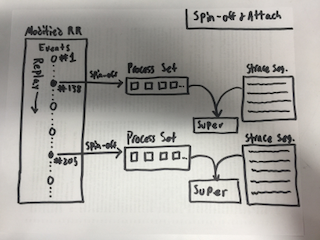
\includegraphics[scale=.75]{architecture}}
  \caption{Diagram illustrating CrashSimulator's Architecture.  During the
    course of a single rr execution, clone process sets are generated at
    specific rr events.  A CrashSimlator supervisor process attaches to
    these process sets and uses a strace-style system call listing to feed
    subsequent system call activity and inject unusual environmental
    conditions.}
  \label{figure:architecture}
\end{figure}

As can be seen in Figure~\ref{figure:architecture},
our implementation of CrashSimulator uses a combination of a modified
version of {\tt rr}, a
record-and-replay debugger, and our own process supervisor
to accomplish the above.
During testing we rely on {\tt rr}
to store the information necessary to perform the bulk of
replay that must take place before the application reaches the point in
execution where testing will be performed.  When this point is reached we
take advantage of {\tt rr's} ``diversion session'' capability to create a
copy of the set of processes being replayed.  Our modifications
allow this process set to be liberated from {\tt rr} so that our
CrashSimulator process supervisor can take over replay responsibilities.

Process sets generated by {\tt rr} are created in a stopped state and
remain until they are attached to and utilized by a CrashSimulator
supervisor.  Each process set has its own supervisor process to inject
its configured environmental anomaly.  The
supervisor wakes up the process set it is managing and simulates any
subsequent system calls it makes.  The data necessary for this
simulation is
supplied as a system call listing formatted after the style of {\tt strace}
output, that describes the results and side effects for each system
call. The output is engineered in such a way to contain the
elements required to reflect the
desired environmental anomaly.  Supervisors can complete this
process independently of one another, which lends a
high degree of speed and
parallelism to the whole CrashSimulator testing process.

\subsection{Improving the CrashSimulator's Capabilities}

CrashSimulator's users are able to improve its capabilities through
the addition of new anomalies.  This process involves identifying a new
anomaly, transforming it into a set of system call results and side
effects, and implementing a mutator script that CrashSimulator can use in
testing applications.

\subsubsection{Anomaly Identification} \label{subsec:anomalyidentification}

The first step in adding a new anomaly to CrashSimulator is to identify the
environmental condition that might cause an application to fail.
Anomalies can be located and isolated via a number of methods. One source
are the public bug trackers of projects available on the web.
Identifying anomalies in this fashion is ideal when determining
whether or not an application is vulnerable to a widely publicized bug.
Additionally, some tools exist that can discover environmental conditions
that might cause problems
for applications
running in the target environment.  This
work utilized the results of both NetCheck~\cite{Zhuang_NSDI_2014} and
CheckAPI~\cite{rasley2015detecting}
to develop some of the
anomalies used in our evaluation.

Anomalies can also be found around more complex operations.  In this case
it is useful to compare how several applications implement the same
operation.  For example, moving files
around in a filesystem is an extremely common operation that, on face
value, seems fairly simple to carry out.  In reality, things become
complex quickly once a few implementation details are taken into account:
namely limitations in Linux's {\tt rename()} system call and the way
Linux's directory hierarchy can abstract away complicated device
configurations.

Trivial cases of moving a file (i.e. those where the source and destination
are on the same device) are accomplished using the {\tt rename()} system
call.  In cases where the source and destination are not on the same device
this system call fails and the application must handle the operation
manually. This means that \emph{any} application that moves files around on
a Linux system must be able to deal with a situation in which some part of
the directory structure may physically reside on a different device.
We examined several popular applications that move files around and
determined that the most thorough example of the operation was carried out
by
the GNU Coreutils {\tt mv} command.  Using this application as our
``gold standard''  we implemented several mutators that
could modify the result of the initial call to {\tt rename} and the
type of the file being removed as represented in the results of a system
call in the {\tt stat} family.
In our evaluation we will discuss how this work found many applications
do not handle the above situations correctly

\subsubsection{Converting Anomalies to System Call Sequences}

Once a new anomaly has been identified, it is distilled into a
representative set of system call results and side effects.
This process involves examining the
system calls made by an application running in the anomalous environment
and selecting a set of modifications that, when applied to a recording,
simulate the presence environmental condition in question.
This process requires manual effort and expertise.  However,
much like
the effort involved in constructing a unit test to check for correct
behavior in a piece of code, this initial outlay of
user skill and effort will be paid back, as it is
used repeatedly over time to test many different applications.

As a more concrete example of the above, consider an anomaly
involving unusual file types we will later address in our evaluation of
CrashSimulator.
This anomaly appears when a call to {\tt stat()} or a similar system
call returns a structure with a {\tt st\_mode}
member containing an unexpected
value. Consider the line of {\tt strace} output representing a call to {\tt
  fstat()}:
\begin{quote}
  {\tt 8936  fstat64(3, \{st\_dev=makedev(0, 40), st\_ino=54993216, st\_mode=S\_IFREG ...\}) = 0}
\end{quote}
The third member of the returned structure indicates that the file is a
regular file by showing that {\tt st\_mode} flag is set in the {\tt st\_mode}
member.  CrashSimulator can mutate this  line to the following:

\begin{quote}
  {\tt 8936  fstat64(3, \{st\_dev=makedev(0, 40), st\_ino=54993216, st\_mode=S\_IFCHR ...\}) = 0}
\end{quote}

The trace containing this modified line can then be replayed in order to
test how the application responds when a file that is expected to be
regular is actually a character device. In our evaluation, we further
explore the behavior of applications as they encounter other possible valid
values of {\tt st\_mode} in the course of testing.

\subsubsection{Implementation Details}
\preston{I am struggling with where to put this information.  Maybe it
should go at the beginning of the evaluation?}
To be able to evaluate how CrashSimulator performs, a series of tests were
conducted using a prototype build on {\tt rr} version 5.2.0 running on a
32-bit Linux kernel running distributed with  Ubuntu 16.04 LTS.  Our
modifications to {\tt rr} were carried out in C++ and the CrashSimulator
supervisor was implemented in ZZZZ lines of Python 2.7 code with a YYYY
line C extension that allows it to interact with processes using the {\tt
Ptrace} API.  This version of CrashSimulator is available as a Docker
container and, due to some operating system configuration being necessary,
is most easily installed in this fashion.

For a test environment, we chose
a vmware virtual machine running version of CrashSimulator described above.
We ran the tests on a 1.7 gHz
core i7 system with 8GB of RAM. Our implementation used {\tt ptrace} to
interpose on the running program and interject anomalous behavior into its
execution.  To our knowledge, the only major negative impact of
these design choices was that the use of {\tt ptrace} and Python did slow
down our
prototype's performance.  On the positive side, it simplified construction.
As will be discussed later, much of this performance
degradation is offset by the highly asynchronous fashion in which our
prototype can execute tests.
